\documentclass[conference,letterpaper]{IEEEtran}
\usepackage[T1]{fontenc}
\usepackage{amsmath,amssymb,booktabs,array,cite,xcolor,capt-of}
\usepackage{tikz,pgfplots,pgfplotstable}
\pgfplotsset{compat=1.18}
\setcounter{dbltopnumber}{2}
\renewcommand{\dbltopfraction}{0.8}
\renewcommand{\textfraction}{0.1}
\usepgfplotslibrary{groupplots}
\usetikzlibrary{arrows.meta,positioning,calc,decorations.pathreplacing}
\usepackage{hyperref}
\newcommand{\StageVsShuffleOne}{1.462}
\newcommand{\RoundVsShuffleOne}{1.520}
\newcommand{\StageVsScalarOne}{5.258}
\newcommand{\RoundVsScalarOne}{5.467}
\newcommand{\RoundVsPqrvOne}{4.742}
\newcommand{\ShuffleVsPqrvOne}{3.120}
\newcommand{\PointerVsScalarOne}{4.840}
\newcommand{\StageVsShuffleEight}{1.552}
\newcommand{\RoundVsShuffleEight}{1.583}
\newcommand{\StageVsScalarEight}{3.646}
\newcommand{\RoundVsScalarEight}{3.719}
\newcommand{\RoundVsPqrvEight}{3.074}
\newcommand{\ShuffleVsPqrvEight}{1.942}
\newcommand{\PointerVsScalarEight}{5.109}
\newcommand{\RoundVsPointerOne}{1.130}
\newcommand{\StageVsPointerOne}{1.087}
\newcommand{\PointerVsRoundEight}{1.374}
\newcommand{\PointerVsStageEight}{1.401}
\newcommand{\BatchScalar}{4.98}
\newcommand{\BatchPqrv}{5.23}
\newcommand{\BatchShuffle}{3.25}
\newcommand{\BatchStage}{3.45}
\newcommand{\BatchRound}{3.39}
\newcommand{\BatchPointer}{5.26}
\newcommand{\KemScalarOne}{28.45}
\newcommand{\KemScalarEight}{45.67}
\newcommand{\KemPqrvOne}{24.67}
\newcommand{\KemPqrvEight}{37.75}
\newcommand{\KemShuffleOne}{7.91}
\newcommand{\KemShuffleEight}{19.44}
\newcommand{\KemStageOne}{5.41}
\newcommand{\KemStageEight}{12.53}
\newcommand{\KemRoundOne}{5.20}
\newcommand{\KemRoundEight}{12.28}
\newcommand{\KemPointerOne}{5.88}
\newcommand{\KemPointerEight}{8.94}
\newcommand{\PermStageLoopOne}{2052}
\newcommand{\PermStageLoopEight}{482}
\newcommand{\PermStageExpOne}{1582}
\newcommand{\PermStageExpEight}{387}
\newcommand{\PermRoundOne}{499}
\newcommand{\PermRoundEight}{118}
\newcommand{\FusionPrimOne}{3.168}
\newcommand{\FusionPrimEight}{3.291}
\newcommand{\FusionAppOne}{1.028}
\newcommand{\FusionAppEight}{1.033}
\newcommand{\FusionAppOnePct}{2.8}
\newcommand{\FusionAppEightPct}{3.3}
\newcommand{\PermStagePct}{5.0}
\newcommand{\SpongeStagePct}{11.7}
\newcommand{\NttStagePct}{2.3}
\newcommand{\PolyStagePct}{4.5}
\newcommand{\OtherStagePct}{76.5}
\newcommand{\PermRoundPct}{1.3}
\newcommand{\SpongeRoundPct}{12.9}
\newcommand{\NttRoundPct}{2.4}
\newcommand{\PolyRoundPct}{4.7}
\newcommand{\OtherRoundPct}{78.8}
\newcommand{\PermPointerPct}{0.5}
\newcommand{\SpongePointerPct}{26.8}
\newcommand{\NttPointerPct}{2.1}
\newcommand{\PolyPointerPct}{4.2}
\newcommand{\OtherPointerPct}{66.4}
\newcommand{\ProbeMinPct}{6.6}
\newcommand{\ProbeMaxPct}{8.3}
\newcommand{\NttPairVsShuffleFwdOne}{2.84}
\newcommand{\NttPairVsShuffleInvOne}{2.60}
\newcommand{\NttPairVsSmemFwdOne}{1.37}
\newcommand{\NttPairVsSmemFwdEight}{1.53}
\newcommand{\NttMulVsCFwdOne}{1.37}
\newcommand{\NttPairVsCFwdOne}{3.89}
\newcommand{\NttKemPairVsShuffleOnePct}{2.6}
\newcommand{\NttKemPairVsShuffleEightPct}{8.2}
\newcommand{\NttKemPairVsSmemOnePct}{1.0}
\newcommand{\NttKemPairVsSmemEightPct}{4.9}
\newcommand{\HalfBankMaxCyclePct}{0.041}
\newcommand{\HalfBankLutSave}{14,767}
\newcommand{\HalfBankLutSavePct}{4.1}
\newcommand{\HalfBankFfSave}{1,565}
\newcommand{\HalfBankDspSave}{16}
\newcommand{\StageLutThirtyTwoPct}{1.129}
\newcommand{\StageFfThirtyTwoPct}{1.300}
\newcommand{\StageWnsThirtyTwo}{0.004}
\newcommand{\RoundLutThirtyTwoPct}{0.898}
\newcommand{\RoundFfThirtyTwoPct}{4.755}
\newcommand{\RoundWnsThirtyTwo}{0.007}
\newcommand{\StageLutSixtyFourPct}{0.880}
\newcommand{\StageFfSixtyFourPct}{1.789}
\newcommand{\StageWnsSixtyFour}{-0.148}
\newcommand{\RoundLutSixtyFourPct}{0.451}
\newcommand{\RoundFfSixtyFourPct}{2.617}
\newcommand{\RoundWnsSixtyFour}{-0.013}
\newcommand{\RvSixtyFourLutRatio}{1.94}
\newcommand{\NttHierLut}{5,624}
\newcommand{\NttHierFf}{5,155}
\newcommand{\NttHierDsp}{16}
\newcommand{\StageHierLut}{838}
\newcommand{\StageHierFf}{2,023}
\newcommand{\RoundHierLut}{2,343}
\newcommand{\RoundHierFf}{6,126}
\newcommand{\RvSixtyFourStageInstrPct}{7.0}
\newcommand{\RvSixtyFourStageMOnePct}{4.1}
\newcommand{\RvSixtyFourStageMEightPct}{-0.4}
\newcommand{\RvSixtyFourRoundInstrPct}{5.7}
\newcommand{\RvSixtyFourRoundMOnePct}{3.0}
\newcommand{\RvSixtyFourRoundMEightPct}{+0.2}
\newcommand{\ScalarKeccakSharePct}{66}
\newcommand{\ScalarNttSharePct}{13}
\newcommand{\MicroPermScalarC}{37,154}
\newcommand{\MicroPermPqrv}{24,782}
\newcommand{\MicroPermSgFive}{15,910}
\newcommand{\MicroPermShuffle}{6,753}
\newcommand{\MicroPermStage}{390}
\newcommand{\MicroPermRound}{120}
\newcommand{\MicroShuffleVsPqrv}{3.7}
\newcommand{\MicroStageVsShuffle}{17.3}
\newcommand{\MicroRoundVsShuffle}{56.3}
\newcommand{\BackendStageLutDelta}{4,031}
\newcommand{\BackendStageLutPct}{1.22}
\newcommand{\BackendStageFfDelta}{1,968}
\newcommand{\BackendStageFfPct}{0.73}
\newcommand{\BackendStageHierLut}{902}
\newcommand{\BackendStageHierFf}{2,025}
\newcommand{\BackendRoundLutDelta}{2,180}
\newcommand{\BackendRoundLutPct}{0.66}
\newcommand{\BackendRoundFfDelta}{6,399}
\newcommand{\BackendRoundFfPct}{2.39}
\newcommand{\BackendRoundHierLut}{2,503}
\newcommand{\BackendRoundHierFf}{6,130}
\newcommand{\BackendPointerLutDelta}{11,221}
\newcommand{\BackendPointerLutPct}{3.39}
\newcommand{\BackendPointerFfDelta}{3,220}
\newcommand{\BackendPointerFfPct}{1.20}
\newcommand{\BackendPointerHierLut}{10,414}
\newcommand{\BackendPointerHierFf}{4,556}
\newcommand{\PointerVsRoundLutDelta}{5.1}
\newcommand{\IpcScalarEight}{0.49}
\newcommand{\IpcScalarOne}{0.099}
\newcommand{\IpcPqrvEight}{0.55}
\newcommand{\IpcPqrvOne}{0.106}
\newcommand{\IpcShuffleEight}{0.28}
\newcommand{\IpcShuffleOne}{0.086}
\newcommand{\IpcStageEight}{0.28}
\newcommand{\IpcStageOne}{0.081}
\newcommand{\IpcRoundEight}{0.27}
\newcommand{\IpcRoundOne}{0.080}
\newcommand{\IpcPointerEight}{0.47}
\newcommand{\IpcPointerOne}{0.090}
\newcommand{\StageLutDeltaThirtyTwo}{2,494}
\newcommand{\StageFfDeltaThirtyTwo}{1,714}
\newcommand{\RoundLutDeltaThirtyTwo}{1,985}
\newcommand{\RoundFfDeltaThirtyTwo}{6,267}
\newcommand{\RoundPerLutVsStage}{5.1}
\newcommand{\InstrScalarEight}{22.57}
\newcommand{\InstrScalarOne}{2.82}
\newcommand{\InstrPqrvEight}{20.90}
\newcommand{\InstrPqrvOne}{2.61}
\newcommand{\InstrShuffleEight}{5.44}
\newcommand{\InstrShuffleOne}{0.68}
\newcommand{\InstrStageEight}{3.49}
\newcommand{\InstrStageOne}{0.44}
\newcommand{\InstrRoundEight}{3.33}
\newcommand{\InstrRoundOne}{0.42}
\newcommand{\InstrPointerEight}{4.22}
\newcommand{\InstrPointerOne}{0.53}
\newcommand{\ModelGapPct}{0.17}


\definecolor{cBlue}{HTML}{315C85}
\definecolor{cTeal}{HTML}{00867D}
\definecolor{cOrange}{HTML}{D28527}
\definecolor{cPurple}{HTML}{873E75}
\definecolor{cGold}{HTML}{D18B24}
\newcommand{\Mont}{\operatorname{Mont}}
\newcommand{\code}[1]{\texttt{#1}}
\makeatletter
\newcommand{\tablerows}[1]{\@@input #1 }
\makeatother
\hypersetup{colorlinks=true,allcolors=cBlue,
 pdftitle={Communication-Matched Warp Collectives for ML-KEM and ML-DSA on a RISC-V SIMT GPU},pdfauthor={Anonymous authors}}

\title{Communication-Matched Warp Collectives for\\
ML-KEM and ML-DSA on a RISC-V SIMT GPU}
\author{\IEEEauthorblockN{Anonymous Authors}}

\begin{document}
\maketitle

\begin{abstract}
ML-KEM and ML-DSA share Keccak and number-theoretic transforms (NTTs), yet
their useful parallelism has incompatible communication: Keccak repeatedly
reduces and permutes a 25-word state, while an NTT exchanges coefficient pairs
at power-of-two distances. We present communication-matched warp collectives
that keep both states in ordinary lane registers of an RV32 RISC-V GPU. The
instructions are stateless, use standard source vectors and single-destination
writeback, and implement fixed Keccak neighborhoods or paired NTT butterflies.
A serialized modular unit shares its routing and multiplier bank across the
16-bit ML-KEM and 32-bit ML-DSA datapaths. A 200-MHz V80 evaluation covers all
six standardized parameter sets against a matched, optimized cooperative
software mapping. Stage, shared NTT, and arithmetic reuse accelerate single
ML-KEM requests (KeyGen--Encaps--Decaps) by
\KemParameterMinOne{}--\KemParameterMaxOne{}$\times$ and ML-DSA requests
(KeyGen--Sign--Verify) by \DsaParameterMinOne{}--\DsaParameterMaxOne{}$\times$;
eight-request batches gain \ParameterMinEight{}--\ParameterMaxEight{}$\times$.
A separate five-point bank sweep supports two multipliers: this design removes
\BankTwoNttDspSaved{}\% of NTT-hierarchy DSPs at a
\BankTwoNttPenalty{}\% NTTBF test-cycle and at most
\BankTwoEndToEndMax{}\% request penalty in middle-set Pointer controls. The results show that GPU
cryptographic hardware must be sized at request scope, not by primitive peak
throughput.
\end{abstract}

\begin{IEEEkeywords}
post-quantum cryptography, ML-KEM, ML-DSA, Keccak, NTT, SIMT, RISC-V
\end{IEEEkeywords}

\section{Introduction}
The standardization of ML-KEM and ML-DSA gives post-quantum key establishment
and digital signatures a common deployment target~\cite{fips203,fips204}.
Although the two schemes provide different services, both repeatedly invoke
SHA-3/SHAKE and polynomial arithmetic. Efficient implementations must also
execute sampling, encoding, and, for signatures, input-dependent rejection
loops. Accelerating an isolated transform or permutation is therefore
insufficient: the useful outcome is lower latency or higher throughput for a
complete cryptographic request, including the surrounding computation.

A programmable GPU offers two levels of parallelism for these workloads.
Threads can cooperate within a polynomial or a hash state, while independent
warps process different requests. GPU implementations of Kyber and Dilithium
already exploit this structure through register reuse, kernel fusion,
batching, and cooperative scheduling~\cite{hikyber,cudilithium}. ML-Cube
further combines GPU execution and machine-learning accelerators, including
a 25-thread Keccak mapping~\cite{mlcube}. These results motivate a complementary
question for an extensible SIMT processor: which remaining work merits
specialized hardware once the software already exploits warp parallelism?

Our starting point is the cost that remains after software cooperation.
On the 200-MHz V80, instrumented complete requests in our cooperative
software baseline attribute \MotivationKemKeccak{}\%/\MotivationDsaKeccak{}\%
of request cycles to Keccak-f and \MotivationKemNtt{}\%/\MotivationDsaNtt{}\% to NTT/INTT for
ML-KEM-768/ML-DSA-65 (Fig.~\ref{fig:motivation}). Both families therefore
remain useful specialization targets. This baseline keeps Keccak and NTT
state in lane registers, with parallel sampling, encoding, and auxiliary
arithmetic enabled identically in every hardware comparison. Our reported
gains measure specialization beyond that software mapping.

The obstacle is not a lack of arithmetic parallelism but the cost of making
operands meet. Each NTT layer contains 128 independent butterflies. With
coefficients distributed across lane registers, some partners lie in the same
lane and others in lanes separated by an XOR distance. Keccak-f[1600] instead
couples 25 64-bit words through column reductions, fixed permutations, and
row-neighbor logic~\cite{fips202}. Generic shuffles express both patterns, but
introduce instructions and dependencies at each exchange. Keeping the state
in registers removes intermediate memory traffic without removing these
communication costs. The two primitives thus favor different internal
connections even when they share the same architectural register interface.

Prior hardware addresses parts of this problem at other boundaries.
RISC-V software optimization~\cite{pqrv} and finite-field instruction
extensions~\cite{alkim,bevin} reduce arithmetic cost; RISQ-V and Nannipieri
et al. add coarser polynomial operations to scalar cores~\cite{risqv,nannipieri}.
Configurable lattice processors such as Sapphire and KaLi already reuse
resources across protocols~\cite{sapphire,kali}, while KiD explicitly unifies
Kyber/Dilithium NTT multiplication~\cite{kid}. Full-protocol FPGA accelerators
also exploit request batching~\cite{highvolume}. Sharing arithmetic is therefore
established; the issue here is how shared arithmetic consumes distributed
SIMT operands and returns results through an existing GPU pipeline.

The hash interface presents a related choice. Prior work quantifies how
state transfers and sponge input/output affect hardware hashing
performance~\cite{karl}. Recent RISC-V extensions retain hash state in private
registers~\cite{horcrux}; a published patent also describes a Keccak round
executed collectively by a warp~\cite{collectivepatent}. Building on these
interfaces, we study the constraints of an RV32 SIMT core: handling 64-bit
state with 32-bit destinations, preserving per-warp dependency tracking, and
selecting the instruction granularity at complete-request scope. A faster
permutation can have little effect once sampling, sponge I/O, or polynomial
work limits execution.

We address three coupled design constraints. First, collective operations
must fit ordinary issue and writeback: an NTT butterfly logically has three
inputs and two outputs, while a Keccak step mixes values from many lanes.
Second, ML-KEM's 16-bit and ML-DSA's 32-bit coefficients require different
reductions without duplicating the entire modular datapath. Third, provisioning
all 16 pair products in parallel may waste resources when other instructions
or warps hide their latency. Neither an isolated primitive benchmark nor a
comparison against scalar C resolves these constraints.

We implement \emph{communication-matched warp collectives} in
Vortex~\cite{vortex}. The state remains in ordinary GPRs, and each instruction
replaces a fixed communication step together with its arithmetic
(Fig.~\ref{fig:thesis}). Two lanes jointly execute one NTT butterfly, compute
one Montgomery product, and each receive one result. A shared serialized
multiplier bank handles both moduli and also serves lane-local products.
Keccak exposes either three stage operations or one fused round, with
explicit low/high outputs on RV32. Every instruction returns a single
architectural destination vector and retains no cryptographic state between
instructions. We compare these register interfaces with a memory-coupled
permutation engine and size the hardware using complete requests.

The resulting Stage-plus-NTT design, including modular-arithmetic reuse,
accelerates complete single-request ML-KEM by
\KemParameterMinOne{}--\KemParameterMaxOne{}$\times$ and ML-DSA by
\DsaParameterMinOne{}--\DsaParameterMaxOne{}$\times$ over matched cooperative
software on a 200-MHz Alveo V80. All six standardized parameter sets are
covered. NTT specialization provides additional request-level gains after
Keccak acceleration. A separate bank sweep finds that two multipliers replace
16 with at most \BankTwoEndToEndMax{}\% request-cycle increase in
its middle-set Pointer controls. Our contributions are:
\begin{itemize}
\item A stateless SIMT instruction interface for Keccak neighborhoods and
XOR-paired NTT butterflies, with ordinary operand tracking and one destination
per lane; controlled Stage, Round, and Pointer comparisons establish the
importance of the execution boundary.
\item A shared K/D modular unit that combines pair routing, modulus-specific
reduction, and a serialized multiplier bank. It supports forward/inverse NTT
and reuses the same arithmetic outside transforms without private polynomial
storage.
\item A complete-library, six-parameter FPGA evaluation with matched software
baselines and separate Keccak, NTT, and arithmetic ablations. Concurrency and
five-point multiplier sweeps connect primitive performance to request latency,
batch throughput, and routed hardware cost.
\end{itemize}

\section{Background and Motivation}
\label{sec:motivation}
\subsection{PQC Workloads and Common Primitives}
ML-KEM establishes keys; ML-DSA provides digital signatures~\cite{fips203,fips204}.
Both use NTT/INTT for polynomial products and Keccak-f[1600] through
SHA-3/SHAKE for hashing and sampling~\cite{fips202}. Their polynomials
have 256 coefficients, with
$q_K=3329$ and $q_D=8380417$; our library mappings use 16-bit KEM and
32-bit DSA coefficients. Keccak updates a $25\times64$-bit state on RV32.
Requests also include encoding and signing retries.

Figure~\ref{fig:motivation} profiles correct cooperative software A on V80
at 200 MHz with one active warp. Complete requests include KeyGen, Encaps,
and Decaps for KEM, and KeyGen, Sign, and Verify for DSA. We use one KEM KAT
input and 32 DSA inputs, with one warmup and five measurements per version.
Each operation is timed separately within its complete request.

Disjoint Keccak-f and NTT/INTT intervals are summed across the measured
requests and divided by their instrumented total cycles. Keccak timing
covers KEM's in-register permutation and DSA's permutation wrapper; the
latter includes dispatch and state transfer. Sponge absorption and extraction
remain in Other. Relative to matched controls without these additional phase
probes, profiling adds \MotivationKemOverheadMax{}\% for KEM and
\MotivationDsaOverheadMin{}--\MotivationDsaOverheadMax{}\% across DSA inputs.
The plot retains this overhead and identifies major costs rather than an
exact uninstrumented breakdown.

\begin{figure}[t]
\centering\begin{tikzpicture}[x=1mm,y=1mm,font=\fontsize{8}{9}\selectfont]
\path[use as bounding box] (0,0) rectangle (88.5,35);
\pgfplotstableread{assets/motivation_profile.dat}\motivationdata

\foreach \tick in {0,25,50,75,100}{
  \pgfmathsetmacro{\xx}{21+.65*\tick}
  \draw[black!10,line width=.3pt] (\xx,7)--(\xx,25.5);
  \draw[black!65,line width=.35pt] (\xx,7)--(\xx,6.2);
  \node at (\xx,4.5) {\tick};
}
\draw[black!65,line width=.35pt] (21,7)--(86,7);

\foreach \row/\name/\yy in {0/{ML-KEM-768}/21.5,1/{ML-DSA-65}/12.5}{
  \node[anchor=west,inner sep=0pt] at (.5,\yy) {\name};
  \pgfplotstablegetelem{\row}{keccak}\of{\motivationdata}
  \pgfmathsetmacro{\keccak}{\pgfplotsretval}
  \pgfplotstablegetelem{\row}{ntt}\of{\motivationdata}
  \pgfmathsetmacro{\ntt}{\pgfplotsretval}
  \pgfplotstablegetelem{\row}{other}\of{\motivationdata}
  \pgfmathsetmacro{\other}{\pgfplotsretval}
  \pgfmathsetmacro{\xk}{21+.65*\keccak}
  \pgfmathsetmacro{\xn}{\xk+.65*\ntt}
  \pgfmathsetmacro{\xo}{\xn+.65*\other}
  \path[fill=cBlue] (21,\yy-3) rectangle (\xk,\yy+3);
  \path[fill=cOrange] (\xk,\yy-3) rectangle (\xn,\yy+3);
  \path[fill=black!16] (\xn,\yy-3) rectangle (\xo,\yy+3);
  \draw[white,line width=.4pt] (\xk,\yy-3)--(\xk,\yy+3);
  \draw[white,line width=.4pt] (\xn,\yy-3)--(\xn,\yy+3);
  \node[text=white,inner sep=0pt] at ({(21+\xk)/2},\yy)
    {\pgfmathprintnumber[fixed,precision=1,zerofill]{\keccak}};
  \node[inner sep=0pt] at ({(\xk+\xn)/2},\yy)
    {\pgfmathprintnumber[fixed,precision=1,zerofill]{\ntt}};
  \node[inner sep=0pt] at ({(\xn+\xo)/2},\yy)
    {\pgfmathprintnumber[fixed,precision=1,zerofill]{\other}};
}

\foreach \xx/\shade/\name in {22/cBlue/{Keccak-f},44/cOrange/{NTT/INTT},68/{black!16}/{Other}}{
  \path[fill=\shade] (\xx,30.5) rectangle (\xx+2,32.5);
  \node[anchor=west,inner sep=0pt] at (\xx+3,31.5) {\name};
}
\node[inner sep=0pt] at (53.5,1.4) {Fraction of instrumented request cycles (\%)};
\end{tikzpicture}

\caption{Instrumented complete-request cycle composition of cooperative
software A on the 200-MHz V80.}
\label{fig:motivation}
\end{figure}

\subsection{Warp-Cooperative Execution and Communication}
\label{sec:software-mapping}
Vortex lanes share an instruction stream over private GPRs~\cite{vortex}.
We assign one primitive to a 32-lane warp and independent requests to
resident warps. Figure~\ref{fig:thesis} shows the resulting communication.
Lane $l$ holds eight coefficients $a[l+32k]$, $0\le k<8$. The first three
forward NTT layers pair registers locally; later layers pair lanes
$l\mathbin{\mathrm{xor}}d$, with $d=16,8,4,2$ for ML-KEM and additionally
$d=1$ for ML-DSA. Inverse traversal reverses this progression.

\begin{figure}[t]
\centering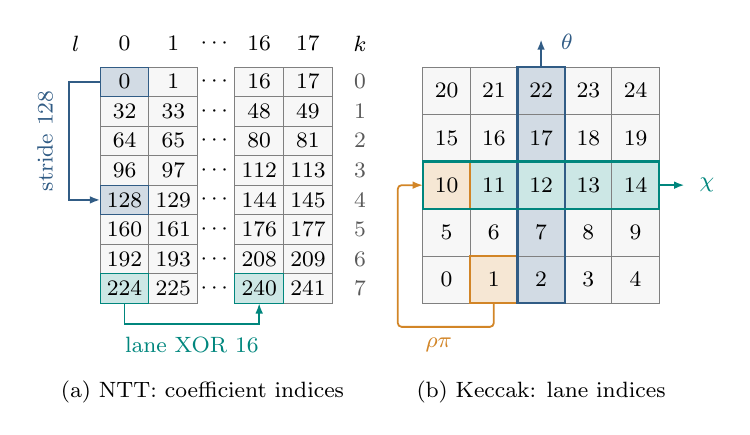
\begin{tikzpicture}[x=1cm,y=1cm,font=\fontsize{8.5}{9.5}\selectfont,
  edge/.style={line width=.65pt,-{Latex[length=1.3mm]}},
  cell/.style={draw=black!50,line width=.35pt}]
\path[use as bounding box] (-.12,-.04) rectangle (8.70,4.78);
\begin{scope}[yshift=3mm]
\node[anchor=east] at (.66,4.28) {$l$};
\foreach \x/\lane in {.80/0,1.42/1,2.51/16,3.13/17}{
  \node at (\x+.31,4.28) {\lane};
  \foreach \k in {0,...,7}{
    \pgfmathtruncatemacro{\coef}{\lane+32*\k}
    \draw[cell,fill=black!3] (\x,3.605-.375*\k) rectangle ++(.62,.375);
    \node at (\x+.31,3.7925-.375*\k) {\coef};
  }
}
\node at (2.275,4.28) {$\cdots$};
\node at (4.10,4.28) {$k$};
\foreach \k in {0,...,7}{
  \node at (2.275,3.7925-.375*\k) {$\cdots$};
  \node[text=black!65] at (4.10,3.7925-.375*\k) {\k};
}
\foreach \k/\coef in {0/0,4/128}{
  \draw[cell,fill=cBlue!22,draw=cBlue] (.80,3.605-.375*\k) rectangle ++(.62,.375);
  \node at (1.11,3.7925-.375*\k) {\coef};
}
\draw[edge,cBlue] (.80,3.7925)--(.40,3.7925)--(.40,2.2925)--(.80,2.2925);
\node[rotate=90,text=cBlue] at (.10,3.0425) {stride 128};
\foreach \x/\coef in {.80/224,2.51/240}{
  \draw[cell,fill=cTeal!20,draw=cTeal] (\x,.98) rectangle ++(.62,.375);
  \node at (\x+.31,1.1675) {\coef};
}
\draw[edge,cTeal] (1.11,.98)--(1.11,.72)--(2.82,.72)--(2.82,.98);
\node[text=cTeal] at (1.965,.45) {lane XOR 16};
\begin{scope}[shift={(4.90,.98)}]
\foreach \x in {0,...,4}{\foreach \y in {0,...,4}{
  \pgfmathtruncatemacro{\lane}{\x+5*\y}
  \def\shade{black!3}
  \ifnum\x=2 \def\shade{cBlue!22}\fi
  \ifnum\y=2 \def\shade{cTeal!20}\fi
  \ifnum\lane=1 \def\shade{cOrange!20}\fi
  \ifnum\lane=10 \def\shade{cOrange!20}\fi
  \draw[cell,fill=\shade] (.60*\x,.60*\y) rectangle ++(.60,.60);
  \node at (.60*\x+.30,.60*\y+.30) {\lane};
}}
\draw[cOrange,line width=.65pt] (.60,0) rectangle (1.20,.60);
\draw[cOrange,line width=.65pt] (0,1.20) rectangle (.60,1.80);
\draw[cBlue,line width=.8pt] (1.20,0) rectangle (1.80,3.00);
\draw[cTeal,line width=.8pt] (0,1.20) rectangle (3.00,1.80);
\draw[edge,cOrange,rounded corners=.5mm] (.90,0)--(.90,-.30)--(-.32,-.30)--(-.32,1.50)--(0,1.50);
\node[text=cOrange] at (.20,-.53) {$\rho\pi$};
\draw[edge,cBlue] (1.50,3.00)--(1.50,3.35);
\node[text=cBlue] at (1.83,3.32) {$\theta$};
\draw[edge,cTeal] (3.00,1.50)--(3.32,1.50);
\node[text=cTeal,anchor=west] at (3.39,1.50) {$\chi$};
\end{scope}
\end{scope}
\begin{scope}[yshift=-1.5mm]
\node[font=\fontsize{8}{9}\selectfont] at (2.10,.30) {(a) NTT: coefficient indices};
\node[font=\fontsize{8}{9}\selectfont] at (6.40,.30) {(b) Keccak: lane indices};
\end{scope}
\end{tikzpicture}

\par\vspace{1.5mm}
\caption{Register placement determines the communication. (a) Selected NTT
lanes: indices 0 and 128 pair within lane 0; 224 and 240 pair across lanes 0
and 16. (b) Keccak uses column parity ($\theta$), a fixed permutation
($\rho\pi$, one edge shown), and row neighbors ($\chi$).}
\label{fig:thesis}
\end{figure}

Keccak places $A[x,y]$ in lane $x+5y$: 25 lanes hold state, and seven are
padding. Each word occupies two RV32 GPRs. This layout exposes column
reductions, fixed rotation/permutation, and row-neighbor accesses. Other
polynomial accelerators use memory rows or private storage~\cite{nttpim,bpntt,cham,zkflex}.

Software baseline A uses these layouts and the same surrounding warp optimizations
as the hardware modes. Register residency removes intermediate state traffic;
fixed exchanges still require dependent shuffle and arithmetic instructions.
These repeated sequences are our specialization target.

\subsection{Challenges for a Register-Collective ISE}
An NTT butterfly consumes two coefficients and a twiddle, producing two
coefficients. The target R-type interface names two source registers and one
destination. Reconciling these operands requires considering their lane
distribution and ordinary writeback. Shared KEM/DSA arithmetic must also
preserve different coefficient widths and native reduction conventions.

Keccak's rotations cross RV32 halves: $\theta$, $\rho\pi$, and a fused
round must derive both outputs from the same old $(L,H)$ state.
Overwriting one half early can corrupt the other; $\chi\iota$ instead
operates on each selected half. Cross-lane operations also require every
referenced producer to participate. Section~\ref{sec:isa} resolves these
operand, dependency, and participation constraints.

\section{Design and Implementation}
\label{sec:design}
We expose the register layouts in Section~\ref{sec:motivation} through a
collective ISA, then implement specialized Keccak and NTT datapaths behind
the core's ordinary operand and writeback interfaces. ML-KEM and ML-DSA share
the modular datapath; Keccak uses a separate fixed-routing unit.

\subsection{Collective ISA}
\label{sec:isa}
On W32, each collective reads two source-register vectors and writes one
ordinary GPR per active lane. State persists in these GPRs: the instruction
neither accesses memory nor retains a private cryptographic context. Keccak
requires all 32 lanes active, with state in lanes 0--24 and zero results in
lanes 25--31. NTT butterflies require a pair-closed mask: either both XOR
partners participate or neither does. Lane-local NTTMUL requires no partner.

Table~\ref{tab:isa} lists the implemented families. Stage is the primary
Keccak design; Round is a fusion comparator. Theta, rho/pi, and Round read
both old RV32 halves $(L,H)$; chi/iota reads its selected half and a
warp-uniform round $r\in[0,23]$. Only lane zero receives the selected
round-constant half. Round encodes $r$ as an immediate. Software preserves
the first result in an ordinary temporary until the second instruction has
captured the same old pair. Round likewise recomputes from
both old halves for each output, without hidden half-round state.

\begin{table}[t]
\caption{RV32 ISA with per-lane operands and results.
Slashes denote separate forms: L/H select half $h$; K/D select modulus
$Q$. NTTBF uses XOR distance $2^s$.}
\label{tab:isa}
\centering\small\setlength{\tabcolsep}{4pt}
\begin{tabular*}{\columnwidth}{@{\extracolsep{\fill}}l c c l@{}}
\toprule
Instruction & $rs_1[l]$ & $rs_2[l]$ & $rd[l]$\\
\midrule
\code{KTHETA.L/H} & $A_{L,l}$ & $A_{H,l}$ & $\theta(A)_h[l]$\\
\code{KRHOPI.L/H} & $A_{L,l}$ & $A_{H,l}$ & $\rho\pi(A)_h[l]$\\
\code{KCHII.L/H} & $A_{h,l}$ & $r$ & $\chi\iota_r(A_h)[l]$\\
\code{KROUND.L/H} $r$ & $A_{L,l}$ & $A_{H,l}$ & $\mathrm{Round}_r(A)_h[l]$\\
\midrule
\code{NTTMUL.K/D} & $a_l$ & $b_l$ & $\Mont_Q(a_l b_l)$\\
\code{NTTBF.CT.K/D} & $a_l$ & $\zeta_l$ & $r_l^{\mathrm{CT}}$, \eqref{eq:ntt-ct}\\
\code{NTTBF.GS.K/D} & $a_l$ & $\zeta_l$ & $r_l^{\mathrm{GS}}$, \eqref{eq:ntt-gs}\\
\bottomrule
\end{tabular*}
\end{table}

For NTTBF, choose pair-low lane $p$ with bit $s$ clear and partner
$h=p\mathbin{\mathrm{xor}}2^s$. The operation uses
$a=a_p$, $b=a_h$, and $\zeta=\zeta_p$; the pair-high $\zeta_h$ is unused.
The forward CT form computes
\begin{equation}
\label{eq:ntt-ct}
t=\Mont_Q(b\zeta),\qquad
(r_p^{\mathrm{CT}},r_h^{\mathrm{CT}})=(a+t,a-t).
\end{equation}
Thus two source vectors express three butterfly inputs, while one destination
vector carries both outputs. Lane-local NTTMUL multiplies its two sources
independently in each active lane. The inverse pair
$(r_p^{\mathrm{GS}},r_h^{\mathrm{GS}})=\mathrm{GS}_Q(a,b,\zeta)$ preserves
the libraries' different conventions:
\begin{align}
\label{eq:ntt-gs}
\mathrm{GS}_K(a,b,\zeta)&=(\mathrm{Barrett}_K(a+b),\Mont_K((b-a)\zeta)),\nonumber\\
\mathrm{GS}_D(a,b,\zeta)&=(a+b,\Mont_D((a-b)\zeta)).
\end{align}
K uses signed low-16-bit operands and arithmetic, then sign-extends its
results; D uses signed 32-bit arithmetic. Montgomery radices are $2^{16}$
and $2^{32}$, respectively. Outputs preserve the libraries' native residue
representations rather than forcing canonical values in $[0,q)$.

Stage and NTT use custom-0 (opcode \code{0x0B}); function fields select
operation, half, modulus, direction, and $s=\log_2d\in[0,4]$ as applicable.
Round uses custom-2 (\code{0x5B}), with $r$ in \code{funct7}. Intrinsics emit
R-type forms through inline \code{.insn}, exposing ordinary register
dependencies to the compiler.

\subsection{Hardware Implementation}
Figure~\ref{fig:architecture} separates core integration, shared K/D
arithmetic, and Keccak's fixed connections. The implementation consumes all
lane operands together and requires 32-wide SIMD and ALU datapaths. It does
not assume physical reuse of the general shuffle network.

\begin{figure*}[t]
\centering% Native 178 x 77 mm.
\definecolor{cDark}{HTML}{343B42}
\definecolor{cGray}{HTML}{CDD3D9}
\begin{tikzpicture}[
 x=1mm,y=1mm,font=\fontsize{8}{9}\selectfont,
 line cap=round,line join=round,
 wire/.style={draw=cDark,line width=.5pt,-{Latex[length=1.1mm,width=.8mm]}},
 bus/.style={wire,line width=.75pt},
 box/.style={draw=cDark!65,line width=.45pt,fill=white,inner sep=1pt,align=center},
 reg/.style={box,fill=cGray!18},
 ctrl/.style={draw=cDark!65,dashed,line width=.45pt,-{Latex[length=1.1mm,width=.8mm]}},
 head/.style={font=\fontsize{8}{9}\selectfont\bfseries,anchor=west},
 mul/.style={circle,draw=cGold,line width=.7pt,fill=cGold!12,
   minimum size=5.6mm,inner sep=0pt,font=\fontsize{12}{12}\selectfont}]
\path[use as bounding box] (0,0) rectangle (178,77);
\node[head] at (.5,75) {(a) Core integration};
\node[head] at (48,75) {(b) Shared NTT (M2)};
\node[head] at (123,75) {(c) Keccak Stage};
\draw[cDark!18,line width=.45pt] (46,3)--(46,71.5);
\draw[cDark!18,line width=.45pt] (121,3)--(121,71.5);

% (a) The original core attachment, widened to keep all five PEs legible.
\node[reg,minimum width=39mm,minimum height=5mm] (issue) at (22,66.5)
  {Issue / scoreboard};
\draw[box] (2.5,49) rectangle (41.5,59.8);
\node at (22,57.8) {Lane GPRs};
\foreach \yy/\rr in {54.6/s1,51.3/s2} {
 \node[anchor=east,inner sep=.5pt] at (7.4,\yy) {$r_{\rr}$};
 \foreach \xx in {8.5,12.2,15.9,19.6,23.3,27,30.7,34.4} {
  \draw[box,draw=cDark!35,fill=cGray!22]
    (\xx,\yy-1.2) rectangle (\xx+3.3,\yy+1.2);
 }
}
\draw[wire] (issue.south)--(22,59.8);
\node[reg,minimum width=39mm,minimum height=5mm] (dispatch) at (22,43.1)
  {PE dispatch};
\draw[bus] (14,49)--(14,45.6);
\draw[bus] (30,49)--(30,45.6);
\foreach \xx/\nn/\tt/\cc in {
 6/Int/INT/cGray,14/MD/MD/cGray,22/Stg/STG/cOrange,
 30/Rnd/RND/cPurple,38/Ntt/NTT/cTeal} {
 \node[box,draw=\cc!90!cDark,fill=\cc!14,minimum width=6.9mm,
   minimum height=7mm,inner sep=.2pt,font=\fontsize{7.5}{8.5}\selectfont\sffamily]
   (pe\nn) at (\xx,33) {\tt};
 \draw[wire] (\xx,40.6)--(pe\nn.north);
 \draw[wire] (pe\nn.south)--(\xx,26.5);
}
\node[reg,minimum width=39mm,minimum height=5mm] (arb) at (22,24)
  {Result arbiter};
\node[reg,minimum width=39mm,minimum height=5mm] (dest) at (22,15.5)
  {$r_d[0{:}31]$};
\draw[bus] (arb.south)--(dest.north);
\draw[ctrl] (issue.east)--(44,66.5)--(44,24)--(arb.east);
\node[rotate=90,fill=white,inner sep=.4pt,text=cDark!80] at (44,51)
  {warp / mask / $r_d$};
\draw[wire] (3,7)--(10,7);
\node[anchor=west,inner sep=1pt,font=\fontsize{7.5}{8.5}\selectfont]
  at (11,7) {data};
\draw[ctrl] (24,7)--(31,7);
\node[anchor=west,inner sep=1pt,font=\fontsize{7.5}{8.5}\selectfont]
  at (32,7) {control};

% (b) Distributed operands, first-beat bypass, shared products and indexed writes.
\begin{scope}[xshift=48mm,font=\fontsize{7.5}{8.5}\selectfont]
\node at (8,70.5) {$r_{s1}$};
\node at (16,70.5) {$r_{s2}$};
\foreach \yy/\ll/\aa/\bb in {65.5/p/a/\zeta,59.5/h/b/{-}} {
 \node[anchor=east,inner sep=.4pt] at (3,\yy) {$\ll$};
 \draw[box,fill=cTeal!9] (4,\yy-2.5) rectangle (12,\yy+2.5);
 \draw[box] (12,\yy-2.5) rectangle (20,\yy+2.5);
 \node at (8,\yy) {$\aa$};
 \node at (16,\yy) {$\bb$};
}
\draw[bus] (12,57)--(12,54);
\draw[box,fill=cTeal!10] (4,54)--(20,54)--(17,49)--(7,49)--cycle;
\node at (12,51.5) {pair / MUL};
\node[circle,draw=cTeal,line width=.65pt,fill=cTeal!8,
 minimum size=5mm,inner sep=0pt] (gspre) at (12,43) {$+/-$};
\draw[bus] (12,49)--(gspre.north);
\node[text=cTeal] at (12,38.5) {GS};
\draw[bus] (18.7,52)--(21,52)--(21,45);
\draw[bus] (gspre.east)--(18,43);
\draw[box,fill=cTeal!8] (18,45.5)--(18,40.5)--(23,42)--(23,44)--cycle;
\draw[cDark,line width=.7pt] (23,43)--(24,43);
\fill[cDark] (24,43) circle (.3mm);
\draw[bus] (24,43)--(24,47)--(25,47);
\node at (31,61) {capture};
\foreach \yy/\txt in {55/{u_i,v_i,c_i},51/{\cdots},47/{u_j,v_j,c_j}} {
 \draw[reg] (25,\yy-2) rectangle (37,\yy+2);
 \node at (31,\yy) {$\txt$};
}
\draw[reg] (25,39)--(37,39)--(35.5,33.5)--(26.5,33.5)--cycle;
\node at (31,36.3) {select};
\draw[bus] (31,45)--(31,39);
\draw[bus] (24,43)--(24,36)--(25.8,36);
\node[fill=white,inner sep=.3pt,rotate=90] at (22.3,37) {beat 0};
\draw[cDark,line width=.7pt] (36.3,36)--(40,36);
\draw[cDark,line width=.7pt] (40,36)--(40,47);
\node[mul] (m0) at (44,47) {$\times$};
\node[mul] (m1) at (44,36) {$\times$};
\draw[bus] (40,47)--(m0.west);
\draw[bus] (40,36)--(m1.west);
\node[text=cGold!85!black] at (44,57.5) {M2};
\node at (44,31) {$32{\times}32$};
\node[box,fill=cGold!9,minimum width=10mm,minimum height=21mm]
 (reduce) at (55,41.5) {$q_K/q_D$\\reduce};
\draw[bus] (m0.east)--(50,47);
\draw[bus] (m1.east)--(50,36);
\node[box,fill=cTeal!10,minimum width=10mm,minimum height=17mm]
 (finish) at (66,42.5) {CT $\pm$\\GS sel.};
\draw[bus] (60,47)--(61,47);
\draw[bus] (60,36)--(61,36);
\draw[bus,draw=cBlue] (38.5,36)--(38.5,65)--(66,65)--(66,51);
\fill[cDark] (38.5,36) circle (.3mm);
\fill[cBlue] (55,65) circle (.3mm);
\draw[bus,draw=cBlue] (55,65)--(55,52);
\node[anchor=west,text=cBlue,inner sep=.3pt] at (56,58) {K-GS};
\draw[cBlue,line width=1pt] (48,63.5)--(48,66.5);
\draw[cBlue,line width=.5pt] (48.7,63.5)--(48.7,66.5);
\node[text=cBlue,inner sep=.3pt] at (53,69) {retained $c_i$: $a$ / sum};
\node[reg,minimum width=18mm,minimum height=7mm] (mode) at (10,27)
 {$d$, mode\\CT / GS / MUL};
\draw[ctrl] (3,30.5)--(2,30.5)--(2,51.5)--(5.4,51.5);
\draw[ctrl] (mode.east)--(21,27)--(21,41.4);
\node[reg,minimum width=12mm,minimum height=4mm] (beat) at (31,25)
 {beat, $d$};
\draw[ctrl] (beat.north)--(31,33.5);
\draw[cDark!65,dashed,line width=.45pt] (beat.east)--(66,25);
\draw[ctrl] (55,25)--(55,31);
\draw[ctrl] (66,25)--(66,34);
% CT illustrates two lane writes; other modes use the same indexed vector.
\node[anchor=west,inner sep=.3pt] at (1,20) {CT assembly};
\foreach \xx/\ww/\vv in {1/9/{\cdots},10/16/{a+t},26/14/{\cdots},40/16/{a-t},56/16/{\cdots}} {
 \draw[reg,fill=cTeal!7] (\xx,8) rectangle (\xx+\ww,14);
 \node at (\xx+.5*\ww,11) {$\vv$};
}
\draw[cDark,line width=.6pt] (71,42.5)--(72,42.5)--(72,17)--(18,17);
\draw[wire] (18,17)--(18,14);
\draw[wire] (48,17)--(48,14);
\draw[ctrl] (37,25)--(40,25)--(40,20)--(33,20)--(33,14);
\node at (18,5) {$p$};
\node at (48,5) {$h=p\mathbin{\mathrm{xor}}d$};
\draw[bus] (72,11)--(72.5,11)--(72.5,1.5)--(63,1.5);
\node[anchor=east,inner sep=.3pt] at (62,1.5) {$r_d[0{:}31]$};
\end{scope}

% (c) Original symbol-level Keccak Stage, cleaned up at native 57 x 77 mm.
% Three alternative paths, not a theta -> rho-pi -> chi-iota sequence.
% A_i denotes 64-bit A[x,i] (the L/H pair); theta consumes both halves.
% u,v,w denote the selected RV32 halves of A[x,y], A[x+1,y], A[x+2,y].
\begin{scope}[font=\fontsize{7.5}{8.5}\selectfont]
\draw[reg] (122,65) rectangle (177.5,70);
\node at (149.75,67.5) {$r_{s1},r_{s2}$: $L,H$ or $X,r$};
\draw[cDark,line width=.55pt] (126.5,63.8)--(175,63.8);
\draw[bus] (149.75,65)--(149.75,63.8);
\draw[wire,draw=cGold] (150.8,63.8)--(150.8,59.8);
\foreach \xx in {162,168.5,173.8} {
 \draw[wire,draw=cTeal] (\xx,63.8)--(\xx,61.3);
}
\foreach \xx/\op/\col in {131.9/\theta/cBlue,147.7/{\rho\pi}/cGold,170.9/{\chi\iota}/cTeal} {
 \node[text=\col,fill=white,inner sep=.4pt,font=\fontsize{8}{9}\selectfont] at (\xx,62.5) {$\op$};
}

% theta: five labeled state words feed one column-parity XOR.
\node[circle,draw=cBlue,line width=.6pt,fill=white,minimum size=4.4mm,inner sep=0pt,font=\fontsize{10}{10}\selectfont] (kparity) at (137.5,52.9) {$\oplus$};
\foreach \yy/\ii/\port in {59.7/0/135,56.3/1/157,52.9/2/180,49.5/3/203,46.1/4/225} {
 \draw[box,draw=cBlue,fill=cBlue!10] (123,\yy-1.45) rectangle (130,\yy+1.45);
 \node[text=cBlue] at (126.5,\yy) {$A_{\ii}$};
 \draw[cBlue,line width=.4pt] (130,\yy)--(kparity.\port);
}
\draw[wire,draw=cBlue] (kparity.south)--(137.5,40);
\node[text=cBlue,fill=white,inner sep=.4pt] at (137.5,46.0) {$C_x$};
% The selected original state word is retained alongside its column parity.
\draw[wire,draw=cBlue] (122.2,65)--(122.2,40);
\node[text=cBlue,fill=white,inner sep=.3pt] at (124,43) {$X$};
\draw[wire,draw=cBlue] (126.5,63.8)--(126.5,61.15);

% rho-pi: the crossed lane wires express a fixed gather, then a rotation.
\draw[box,draw=cGold,fill=cGold!8] (144.5,53.8) rectangle (157.1,59.8);
\foreach \xx/\zz in {146.2/150.8,150.8/155.4,155.4/146.2} {
 \draw[cGold,line width=.55pt] (\xx,59.8)--(\zz,53.8);
}
\node[fill=cGold!8,text=cGold!85!black,inner sep=.2pt,font=\fontsize{9}{10}\selectfont] at (150.8,56.8) {$\pi$};
\draw[wire,draw=cGold] (150.8,53.8)--(150.8,49.4);
\node[box,draw=cGold,fill=cGold!9,minimum width=13mm,minimum height=4.4mm] (krotate) at (150.8,47.2) {$\mathrm{ROL}_{\rho}$};
\draw[wire,draw=cGold] (krotate.south)--(150.8,40);

% chi: three labeled row words feed the actual NOT / AND / XOR network.
\foreach \xx/\vv in {162.0/u,168.5/v,173.8/w} {
 \draw[box,draw=cTeal,fill=cTeal!10] (\xx-2.3,58.3) rectangle (\xx+2.3,61.3);
 \node[text=cTeal] at (\xx,59.8) {$\vv$};
}
\node[circle,draw=cTeal,line width=.6pt,fill=white,minimum size=3.6mm,inner sep=0pt,font=\fontsize{9}{9}\selectfont] (knot) at (168.5,53.5) {$\neg$};
\node[circle,draw=cTeal,line width=.6pt,fill=white,minimum size=3.6mm,inner sep=0pt,font=\fontsize{9}{9}\selectfont] (kand) at (171,49.5) {$\land$};
\node[circle,draw=cTeal,line width=.6pt,fill=white,minimum size=3.6mm,inner sep=0pt,font=\fontsize{9}{9}\selectfont] (kchi) at (165.5,43.5) {$\oplus$};
\draw[wire,draw=cTeal] (168.5,58.3)--(knot.north);
\draw[wire,draw=cTeal] (knot.south)--(168.5,49.5)--(kand.west);
\draw[wire,draw=cTeal] (173.8,58.3)--(173.8,49.5)--(kand.east);
\draw[wire,draw=cTeal] (162,58.3)--(162,43.5)--(kchi.west);
\draw[wire,draw=cTeal] (kand.south)--(171,43.5)--(kchi.east);
\draw[wire,draw=cTeal] (kchi.south)--(165.5,40);
% The separate r operand indexes the round constant; it is not a row word.
\node[box,draw=cTeal,fill=cTeal!9,minimum width=5.4mm,minimum height=3.8mm] (krc) at (174.6,43.5) {RC};
\draw[wire,draw=cTeal] (177.7,65)--(177.7,47)--(174.6,47)--(krc.north);
\node[text=cTeal,fill=white,inner sep=.3pt] at (177.7,54.5) {$r$};
\draw[wire,draw=cTeal] (krc.south)--(174.6,40);

% First register boundary: alternative payloads occupy the same R1 stage.
\draw[reg,fill=cBlue!10] (122,36) rectangle (142.4,40);
\draw[reg,fill=cGold!10] (142.4,36) rectangle (159.1,40);
\draw[reg,fill=cTeal!10] (159.1,36) rectangle (177.5,40);
\node[anchor=west,inner sep=.3pt,font=\fontsize{8}{9}\selectfont] at (122.6,38) {$R_1$};
\node[text=cBlue] at (134.7,38) {$X,C[0{:}4]$};
\node[text=cGold!85!black] at (150.75,38) {$T_{\rho\pi}$};
\node[text=cTeal] at (168.3,38) {$Y,\mathrm{RC}_{\ell}$};

% theta second step: neighboring parities and the retained state word.
\draw[wire,draw=cBlue] (129,36)--(129,33.3);
\draw[wire,draw=cBlue] (138.8,36)--(138.8,33.3);
\node[text=cBlue,fill=white,inner sep=.35pt] at (129,32.4) {$C_{x-1}$};
\node[text=cBlue,fill=white,inner sep=.35pt] at (138.8,32.4) {$C_{x+1}$};
\node[box,draw=cBlue,fill=cBlue!8,minimum width=8mm,minimum height=4.4mm] (krolone) at (138.8,27.3) {$\mathrm{ROL}_1$};
\draw[wire,draw=cBlue] (138.8,31)--(krolone.north);
\node[circle,draw=cBlue,fill=white,line width=.6pt,minimum size=4mm,inner sep=0pt,font=\fontsize{10}{10}\selectfont] (kmix) at (133,21.8) {$\oplus$};
\draw[wire,draw=cBlue] (129,31)--(129,21.8)--(kmix.west);
\draw[wire,draw=cBlue] (krolone.south)--(138.8,21.8)--(kmix.east);
\node[circle,draw=cBlue,fill=white,line width=.6pt,minimum size=4mm,inner sep=0pt,font=\fontsize{10}{10}\selectfont] (kthetaout) at (133,14.3) {$\oplus$};
\draw[wire,draw=cBlue] (kmix.south)--(kthetaout.north);
\draw[wire,draw=cBlue] (123.8,36)--(123.8,14.3)--(kthetaout.west);
\node[text=cBlue,fill=white,inner sep=.4pt] at (123.8,26.3) {$X$};
\draw[wire,draw=cBlue] (kthetaout.south)--(133,10);

% rho-pi bypasses the second arithmetic step; this is a registered pass.
\draw[wire,draw=cGold] (150.8,36)--(150.8,10);
\node[text=cGold!85!black,fill=white,inner sep=.8pt] at (150.8,23.4) {pass};

% chi-iota second step: RC_l is zero except in state lane (0,0).
\draw[wire,draw=cTeal] (163.1,36)--(163.1,33.3);
\draw[wire,draw=cTeal] (174.6,36)--(174.6,33.3);
\node[text=cTeal,fill=white,inner sep=.35pt] at (163.1,32.4) {$Y$};
\node[text=cTeal,fill=white,inner sep=.35pt] at (174.6,32.4) {$\mathrm{RC}_{\ell}$};
\node[circle,draw=cTeal,fill=white,line width=.6pt,minimum size=4mm,inner sep=0pt,font=\fontsize{10}{10}\selectfont] (kiotaout) at (168.3,21.8) {$\oplus$};
\draw[wire,draw=cTeal] (163.1,31)--(163.1,21.8)--(kiotaout.west);
\draw[wire,draw=cTeal] (174.6,31)--(174.6,21.8)--(kiotaout.east);
\draw[wire,draw=cTeal] (kiotaout.south)--(168.3,10);

% Second register boundary and the one-half RV32 destination.
\draw[reg] (122,6) rectangle (177.5,10);
\node[anchor=west,inner sep=.3pt,font=\fontsize{8}{9}\selectfont] at (122.6,8) {$R_2$};
\node at (149.75,8) {selected result};
\draw[bus] (149.75,6)--(149.75,2.3);
\node[anchor=west,inner sep=.5pt] at (152.0,2.5) {$r_d=L'$ or $H'$};
\end{scope}

\end{tikzpicture}

\caption{Core integration and collective datapaths. (a) Dedicated PEs share
operand dispatch and result arbitration with INT and multiply/divide.
(b) Beat zero bypasses capture; later $(u_i,v_i,c_i)$ groups are replayed.
M2 multiplies $u_i v_i$; registered $c_i$ ($a$ or the GS sum) feeds K-GS
reduction and finishing. Op selects CT/GS/MUL. CT slots use
$t=\mathrm{Mont}_Q(b\zeta)$; the vector returns after the last beat.
(c) Three alternative Stage paths cross $R_1/R_2$.
$A_{x,i}=A[x,i]$ combines $L/H$; $X$ is the retained half;
$u,v,w$ are row-neighbor halves. Round index $r$ selects
$\mathrm{RC}_{\ell}$, zero except at lane zero.}
\label{fig:architecture}
\end{figure*}

\subsubsection{Keccak Datapath}
Figure~\ref{fig:architecture}c implements fixed connections among the 25
state lanes. Theta first XOR-reduces each column to $C_x$, then injects
$C_{x-1}\oplus\mathrm{rol}_{64}(C_{x+1},1)$ into that column. Rho/pi uses a
fixed gather and the source word's rotation constant. Chi combines neighboring
words within a row; iota injects the selected constant into word zero.

Stage has two registered steps. The first captures column parity and the
selected input half for theta, the rotated/gathered result for rho/pi, or row
logic and the constant for chi/iota. The second completes theta or constant
injection; rho/pi passes through. These are alternative paths, not a serial
three-operation pipeline. Round instead registers parity, theta, rho/pi, and
chi/iota across four steps. Without stalls, both accept one instruction per
cycle; unit latencies are two and four cycles, respectively, plus one shared
return cycle. Stage requires six RV32 issues per round and Round two.
The separate Pointer comparator loads and stores a 200-byte state through the
LSU rather than using the register-collective interface.

\subsubsection{Shared K/D Modular Datapath}
\label{sec:ntt-hw}
Figure~\ref{fig:architecture}b separates pair preparation, variable
multiplication, modular reduction, and lane-result assembly. K mode
sign-extends its inputs and uses Montgomery reduction for $q_K=3329$; K-GS
additionally multiplies each pair sum by 20159 for Barrett reduction. D uses
the full signed product and its own Montgomery constants for $q_D=8380417$.
Mode selection controls preparation and reduction, while capture, multipliers,
beat scheduling, coefficient bypass, and assembly remain shared. NTTMUL
selects lane-local inputs for the same datapath. Explicit twiddles require no
internal twiddle ROM or transform-layer state.

A bank of $M$ signed $32\times32$ multipliers serializes logical products
without changing the instruction or binary; $M$ counts general product
multipliers, not FPGA DSP blocks. CT and D-GS require $B=16/M$ beats. K-GS
requires $B=32/M$ for twiddle and Barrett products; 32-lane NTTMUL also uses
$32/M$. Inactive pairs do not compress these slots. Figure~\ref{fig:detail}a
shows M2 assigning 16 CT products to eight beats. Products traverse factor
and reduction registers; retained coefficients bypass multiplication into
butterfly finishing.

\begin{figure}[t]
\centering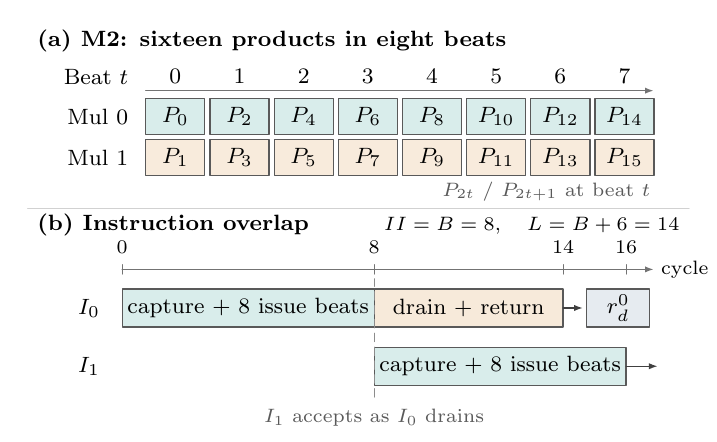
\begin{tikzpicture}[
 x=1mm,y=1mm,font=\fontsize{8}{9}\selectfont,
 line cap=round,line join=round,
 box/.style={draw=black!65,line width=.45pt,fill=white,inner sep=1pt,align=center},
 wire/.style={draw=black!75,line width=.5pt,-{Latex[length=1.1mm,width=.8mm]}},
 head/.style={font=\fontsize{8}{9}\selectfont\bfseries,anchor=west}]
\path[use as bounding box] (0,0) rectangle (84,49);

\node[head] at (0,47.3) {(a) M2: sixteen products in eight beats};
\node[anchor=east] at (14,42.8) {Beat $t$};
\node[anchor=east] at (14,37.7) {Mul 0};
\node[anchor=east] at (14,32.5) {Mul 1};
\foreach \i in {0,...,7} {
  \pgfmathsetmacro{\xx}{15+8.15*\i}
  \pgfmathtruncatemacro{\even}{2*\i}
  \pgfmathtruncatemacro{\odd}{2*\i+1}
  \node at (\xx+3.75,42.8) {\i};
  \draw[box,fill=cTeal!15] (\xx,35.4) rectangle (\xx+7.5,40.0);
  \draw[box,fill=cOrange!16] (\xx,30.2) rectangle (\xx+7.5,34.8);
  \node at (\xx+3.75,37.7) {$P_{\even}$};
  \node at (\xx+3.75,32.5) {$P_{\odd}$};
}
\draw[wire,draw=black!55] (15,41.0)--(79.5,41.0);
\node[anchor=east,text=black!65,font=\fontsize{7}{8}\selectfont]
  at (80.3,28.2) {$P_{2t}$ / $P_{2t+1}$ at beat $t$};

\draw[black!18,line width=.45pt] (0,26.0)--(84,26.0);

\node[head] at (0,23.9) {(b) Instruction overlap};
\node[anchor=east,font=\fontsize{7.5}{8.5}\selectfont] at (84,23.9)
  {$II=B=8,\quad L=B+6=14$};

\draw[wire,draw=black!55] (12,18.3)--(79.5,18.3);
\foreach \xx/\lab in {12/0,44/8,68/14,76/16} {
  \draw[black!55,line width=.4pt] (\xx,17.7)--(\xx,18.9);
  \node[anchor=south,font=\fontsize{7}{8}\selectfont] at (\xx,19.1) {$\lab$};
}
\node[anchor=west,font=\fontsize{7}{8}\selectfont] at (79.2,18.3) {cycle};

\node[anchor=east] at (10.4,13.4) {$I_0$};
\node[anchor=east] at (10.4,6.0) {$I_1$};
\draw[box,fill=cTeal!15] (12,11.0) rectangle (44,15.8);
\node at (28,13.4) {capture + 8 issue beats};
\draw[box,fill=cOrange!17] (44,11.0) rectangle (68,15.8);
\node at (56,13.4) {drain + return};
\draw[wire] (68,13.4)--(70.5,13.4);
\node[box,fill=cBlue!12,minimum width=8mm,minimum height=4.8mm]
  at (75,13.4) {$r_d^0$};

\draw[box,fill=cTeal!15] (44,3.6) rectangle (76,8.4);
\node at (60,6.0) {capture + 8 issue beats};
\draw[wire] (76,6.0)--(80,6.0);
\draw[black!45,densely dashed,line width=.45pt] (44,2.1)--(44,17.1);
\node[anchor=north,font=\fontsize{7}{8}\selectfont,text=black!65]
  at (44,1.8) {$I_1$ accepts as $I_0$ drains};
\end{tikzpicture}

\caption{M2 serialization. (a) At beat $t$, the multipliers accept pair
products $P_{2t}$ and $P_{2t+1}$, so CT/D-GS use eight beats. (b) $I_1$
begins as $I_0$ drains: the initiation interval is 8 cycles and the
acceptance-to-commit latency is 14 cycles. K-GS/NTTMUL use 16 beats.}
\label{fig:detail}
\end{figure}

\subsubsection{Execution Control and Core Integration}
Figure~\ref{fig:architecture}a places Stage, Round, and NTT beside the
integer and multiply/divide PEs. Decode names the ordinary source and
destination registers for scoreboard tracking; ALU dispatch selects the PE,
and a round-robin result arbiter feeds the existing commit path. No additional
register-file port or private architectural register bank is required.

Figure~\ref{fig:detail}b shows the resulting instruction overlap. A serialized
NTT instruction feeds the first product group and captures the
remaining groups, retained coefficients, and warp metadata on its first
handshake. Saved operands feed subsequent beats; a new instruction can enter
after those beats launch while its predecessor drains. Warp, destination,
mask, and beat indices follow the products. Indexed assembly collects partial
results and releases one destination vector after the last beat. Backpressure
freezes the serializer, pipeline, and assembly together. Without stalls,
initiation interval is $B$ and latency including the shared return is $B+6$
cycles: M2 CT takes eight beats and 14 cycles. The destination remains pending
in the scoreboard until the vector returns; intermediate beats never update
architectural registers. Other ready warps can issue to available PEs during
this interval. Retained operands and partial results are in-flight state, not
persistent accelerator-private context.

\subsection{Software Integration}
Native hooks preserve the mlkem-native/mldsa-native APIs and byte-exact outputs
across all six parameter sets~\cite{mlkemnative,mldsanative}. Lane zero
broadcasts arguments, enters the cooperative region, and resumes scalar
control afterward. Each resident warp handles one request at a time; the
leader controls allocation and signing rejection. One-shot SHAKE retains state
in registers across absorb, permutation, and squeeze; incremental contexts are
stored between calls. NTT loads eight coefficients per lane and completes the
transform without intermediate memory, using lane-local multiplication or
XOR-paired butterflies as required. Kernels enforce participation and old-half
dependencies.

Transform-external reuse preserves reduction boundaries. DSA pointwise
products use NTTMUL.D; matrix-vector products first accumulate
$L\in\{4,5,7\}$ raw products in 64-bit software, then perform one Montgomery
reduction per coefficient. KEM basemul retains software products and
accumulation, optionally reusing NTTMUL.K for Montgomery correction. Thus reuse
does not replace every raw product with an independently reduced product.

RTL assertions and unit/processor tests cover participation, both moduli, XOR
distances, dependencies, metadata, and backpressure. Library outputs match
portable C byte for byte; SimX models the same beats and stalls, with matched
binaries checked through XRT integration.


\section{Evaluation}
\label{sec:evaluation}
\subsection{Experimental Methodology}
We use a 200-MHz Alveo V80 with one RV32IM Vortex core, eight resident
32-lane warps, and 16 KiB each of instruction cache, write-through data cache,
and local memory. L2/L3 are disabled; the NTT bank has two multipliers.
Vivado 2025.1 produces the FPGA implementations, with OPT3 for independent
core routing. The board clock is checked before and after measurement.

Each request executes KeyGen--Encaps--Decaps for ML-KEM or
KeyGen--Sign--Verify for ML-DSA. All six standardized parameter sets are
covered. A worker is a resident warp processing one request at a time.
Baseline A uses Section~\ref{sec:software-mapping}'s cooperative mapping;
B adds Stage, C adds NTT, D combines both, and E adds NTTMUL outside
transforms. At each worker count, all modes use matched inputs, surrounding
software, zeroization, and board image. Opcode audits verify that A has no
PQC instructions and A/B have no NTT instructions.

Request-batch makespan is measured in on-device cycles from the earliest
request start to the latest completion, including gaps between waves but
excluding host transfers and setup outside this interval.
After one warmup, five runs yield the median $C_X$; speedup is $C_A/C_X$
at matched batch size and worker count. Across 156 configurations, the
five-run range divided by the median has median \BoardRepeatSpreadMedian{}\% and maximum \BoardRepeatSpreadMax{}\%.
Repeated inputs measure timing variation, not the distribution of signing
retries. These runs omit Fig.~\ref{fig:motivation}'s extra phase probes.
All 780 measurements match portable C byte-for-byte. RTL tests cover both
moduli, directions, lane pairing, masks, and backpressure; 60 headline
SimX/XRT pairs retire identical instruction counts, with at most
\HeadlineParityMax{}\% difference in whole-device PERF cycle counts.
Board instruction counts also match XRT.

\begin{table}[t]
\caption{Request batches at 200 MHz, with $N$ requests on $W=N$ workers.
Each request executes KeyGen--Encaps--Decaps (KEM) or
KeyGen--Sign--Verify (DSA). $S_X=C_A/C_X$ uses five-run medians;
$C_E$ is E's batch makespan in Mcycles. Bold marks E.}
\label{tab:requests}
\centering\footnotesize
\begin{tabular*}{\columnwidth}{@{\extracolsep{\fill}}lrrrrrr@{}}
\toprule
Parameter & $N$ & $S_B$ & $S_C$ & $S_D$ & $\mathbf{S_E}$ & $C_E$\\
\midrule
\tablerows{assets/parameter_ablation_rows.tex}
\bottomrule
\end{tabular*}
\end{table}

\subsection{Complete-Request Acceleration}
Table~\ref{tab:requests} reports B--E relative to A. E accelerates
single-request KEM/DSA by
\KemParameterMinOne{}--\KemParameterMaxOne{}$\times$/
\DsaParameterMinOne{}--\DsaParameterMaxOne{}$\times$; at eight requests,
the ranges are \KemParameterMinEight{}--\KemParameterMaxEight{}$\times$/
\DsaParameterMinEight{}--\DsaParameterMaxEight{}$\times$.
Single-request E takes \KemRequestMcyclesMin{}--\KemRequestMcyclesMax{}
Mcycles for KEM and \DsaRequestMcyclesMin{}--\DsaRequestMcyclesMax{} for DSA.

Across all sets and both batch sizes, Stage alone gives
\KemStageMin{}--\KemStageMax{}$\times$/\DsaStageMin{}--\DsaStageMax{}$\times$
for KEM/DSA (A/B). With Stage fixed, NTT adds
\KemNttMin{}--\KemNttMax{}$\times$/\DsaNttMin{}--\DsaNttMax{}$\times$ (B/D).
Arithmetic reuse gives another \DsaArithmeticMin{}--\DsaArithmeticMax{}$\times$
for DSA without new RTL. KEM changes only
\KemArithmeticMin{}--\KemArithmeticMax{}$\times$ (D/E); KEM-768 shows no
improvement. These ratios isolate successive contributions within each
matched case; all headline results use E.

\subsection{Granularity and Arithmetic Capacity}
Archived fusion controls use write-back caching. Relative to equally unrolled
Stage, Round improves XRT permutation throughput by
\FusionOne{}$\times$/\FusionEight{}$\times$ at one/eight warps, but separate
SimX complete-KEM gains are only \FusionKemOne{}$\times$/\FusionKemEight{}$\times$
(no paired XRT run for the latter). An instrumented XRT request spends only
\StagePermPct{}\% in Stage permutation. A fixed-mapping control favors Round
over Pointer by \RoundVsPointerOne{}$\times$ for one request, but Pointer
over Round by \PointerVsRoundEight{}$\times$ for eight: the preferred
interface depends on request scope and concurrency.

\begin{table}[t]
\caption{NTT bank tradeoffs relative to M16. Program cycles use historical
W4T32 NTTBF.K RTL; request overhead is the maximum over W8T32 Pointer
controls (KEM-768/DSA-65, $N=1/8$). NTT counts use independent 200-MHz routing.}
\label{tab:bank}
\centering\footnotesize
\begin{tabular*}{\columnwidth}{@{\extracolsep{\fill}}lrrrrr@{}}
\toprule
& \multicolumn{2}{c}{Cycle increase (\%)} & \multicolumn{3}{c}{NTT hierarchy}\\
\cmidrule(lr){2-3}\cmidrule(l){4-6}
Bank & Program & Max. request & LUT & FF & DSP\\
\midrule
\tablerows{assets/ntt_bank_rows.tex}
\bottomrule
\end{tabular*}
\end{table}

Table~\ref{tab:bank} separates three experiments. NTTBF test cycles include
loads, stores, and loops on historical RV32IMF W4T32 RTL. Request overheads
use RV32IM W8T32 write-back XRT with Pointer fixed, for KEM-768/DSA-65 and
one/eight requests. Resources come from independent 200-MHz routed cores.
Each timing sweep preserves its binary and inputs across banks.
M2 raises NTTBF cycles by \BankTwoNttPenalty{}\% and requests by at most
\BankTwoEndToEndMax{}\%, while removing \BankTwoNttLutSaved{}\% of NTT LUTs,
\BankTwoNttFfSaved{}\% of FFs, and \BankTwoNttDspSaved{}\% of DSPs.
M1 saves only five more core DSPs, increases NTT FFs, and raises test cycles
by \BankOneNttPenalty{}\%. All banks pass 1,044 test vectors and retire
59,534 test instructions, within \BankParityMax{}\% SimX/RTL cycle difference.
The smaller request sensitivity supports M2 in this cohort; it does not
isolate latency hiding or establish Stage+M2 joint optimality.

\subsection{Worker Count and Batch Size}
\begin{figure}[t]
\centering\begin{tikzpicture}
\begin{groupplot}[
 group style={group size=2 by 1,horizontal sep=13mm},
 scale only axis,width=.34\columnwidth,height=29mm,
 axis lines*=left,axis line style={black!65},
 tick label style={font=\fontsize{8}{9}\selectfont},
 label style={font=\fontsize{8}{9}\selectfont},
 title style={font=\fontsize{8}{9}\selectfont,
  at={(.5,0)},anchor=north,yshift=-10mm},
 xmode=log,log basis x=2,xmin=.92,xmax=8.7,
 xtick={1,2,4,8},xticklabels={1,2,4,8},
 xlabel={Workers $W$},
 tick align=outside,major tick length=2pt,
 ymajorgrids=true,grid style={black!12},
 every axis plot/.append style={line width=.8pt,mark size=1.45pt},
 cycle list={{cBlue,mark=*},{cOrange,mark=square*},
 {cPurple,mark=triangle*},{cTeal,dashed,mark=diamond*},
 {black!65,dashed,mark=otimes*},{cGold,dashed,mark=pentagon*}}]
\nextgroupplot[
 title={(a) E throughput},
 ymin=.9,ymax=3.2,ytick={1,2,3},ylabel={Normalized rate},
 legend to name=scalinglegend,
 legend style={font=\fontsize{8}{9}\selectfont,draw=none,
  legend columns=3,legend cell align=left,column sep=3pt,
  /tikz/every even column/.append style={column sep=5pt}}]
\addplot table[x=workers,y=K512]{assets/parameter_occupancy.dat};
\addlegendentry{K512}
\addplot table[x=workers,y=K768]{assets/parameter_occupancy.dat};
\addlegendentry{K768}
\addplot table[x=workers,y=K1024]{assets/parameter_occupancy.dat};
\addlegendentry{K1024}
\addplot table[x=workers,y=D44]{assets/parameter_occupancy.dat};
\addlegendentry{D44}
\addplot table[x=workers,y=D65]{assets/parameter_occupancy.dat};
\addlegendentry{D65}
\addplot table[x=workers,y=D87]{assets/parameter_occupancy.dat};
\addlegendentry{D87}
\nextgroupplot[
 title={(b) E versus A},
 ymin=1.75,ymax=2.45,ytick={1.8,2.0,2.2,2.4},
 yticklabel style={/pgf/number format/fixed,/pgf/number format/precision=1},
 ylabel={Speedup ($\times$)}]
\addplot table[x=workers,y=K512]{assets/parameter_worker_speedup.dat};
\addplot table[x=workers,y=K768]{assets/parameter_worker_speedup.dat};
\addplot table[x=workers,y=K1024]{assets/parameter_worker_speedup.dat};
\addplot table[x=workers,y=D44]{assets/parameter_worker_speedup.dat};
\addplot table[x=workers,y=D65]{assets/parameter_worker_speedup.dat};
\addplot table[x=workers,y=D87]{assets/parameter_worker_speedup.dat};
\end{groupplot}
\path (group c1r1.south west)--(group c2r1.south east)
 node[midway,below=14mm]{\pgfplotslegendfromname{scalinglegend}};
\end{tikzpicture}

\caption{Fixed eight-request workload on the 200-MHz V80.
(a) E throughput relative to E at one worker.
(b) E speedup over software A at the same worker count.
Each worker is one warp; curves use five-run medians.}
\label{fig:scaling}
\end{figure}
Figure~\ref{fig:scaling} fixes eight inputs. With $R_E=8f/C_E$ at
$f=200$ MHz, panel (a) normalizes E throughput to one worker; panel (b)
compares E with A at the same worker count: E retains a \ParameterWorkerSpeedupMin{}--\ParameterWorkerSpeedupMax{}$\times$
advantage across these configurations. One to eight workers increases
E throughput by \ParameterOccupancyMin{}--\ParameterOccupancyMax{}$\times$.
This includes a zeroization-policy change: one worker uses cooperative
zeroization; multiple workers use leader execution, identically for A/E.
Thus the curve does not isolate occupancy. Separately, at eight workers,
extending batches from eight to 64 changes throughput by only
\ParameterBatchMin{}--\ParameterBatchMax{}$\times$; intermediate DSA batches
peak at \ParameterBatchPeak{}$\times$. Synchronized waves and longer input
prefixes combine amortization with input-dependent signing retries.

\subsection{Routed Cost and Design Scope}
\begin{table}[t]
\caption{Independent 200-MHz post-route RV32IM cores with NTT.
Stage, Round, and Pointer add alternative Keccak units.}
\label{tab:cost}
\centering\footnotesize\setlength{\tabcolsep}{3.4pt}
\begin{tabular}{@{}lrrrr@{}}
\toprule
Variant & LUT & FF & DSP & WNS (ns)\\
\midrule
\tablerows{assets/cost_rows.tex}
\bottomrule
\end{tabular}
\end{table}
All Table~\ref{tab:cost} cores close at 200 MHz without routing errors.
NTT-M2 saves \BankTwoCoreLutSaved{}\% whole-core LUTs and
\BankTwoCoreDspSaved{}\% DSPs over NTT-M16. Stage adds \JointStageLutPct{}\% LUTs
to an M2 core that already includes NTT; this is incremental Keccak cost.
Round uses fewer LUTs but more FFs than Stage at M16. The board AFU includes
optional engines (\BoardAfuLuts{} LUTs, \BoardAfuFfs{} FFs,
\BoardAfuDsps{} DSPs; \BoardWns{} ns slack); board ratios compare software
paths within that image. Six-set results validate Stage+M2, while the bank
sweep remains a separate Pointer control. Energy and host-to-host latency
are unmeasured.

\section{Conclusion}
Stateless warp collectives match Keccak neighborhoods and XOR-paired NTT
butterflies to ordinary lane registers. A shared K/D modular datapath
supports both coefficient widths and arithmetic reuse while retaining
single-destination writeback. On a 200-MHz V80, Stage+M2 with reuse accelerates
three-API requests across all six parameter sets by
\ParameterMinOne{}--\ParameterMaxOne{}$\times$ individually and
\ParameterMinEight{}--\ParameterMaxEight{}$\times$ in eight-request batches
over matched cooperative software. Independent routing shows
\BankTwoNttDspSaved{}\% fewer NTT DSPs for M2 than M16; a separate Pointer
control measures at most \BankTwoEndToEndMax{}\% request-cycle overhead.
These results support choosing communication, instruction granularity, and
arithmetic capacity using complete-request cost at the intended concurrency.
Register residency lets these operations coexist with optimized sampling,
encoding, and request scheduling on a programmable SIMT core.

\clearpage
\bibliographystyle{IEEEtran}
\bibliography{references}
\end{document}
